\chapter{Planeamento da Investigação}
\section{Metodologia de Investigação}
A metodologia de investigação utilizada nesta dissertação baseia-se na investigação-ação \cite{somekh2006action}. Esta assenta no princípio de que a procura da solução é baseada no desafio proposto. Desta forma o trabalho desenvolvido pretende dar resposta ao problema identificado, através da compilação de toda a informação proveniente do trabalho de pesquisa efetuado. Este processo culmina no registo de toda a informação relevante, servindo esta de base para a construção de uma solução para o problema.

Posto isto, importa salientar os pontos chave a percorrer tendo em conta uma metodologia de investigação-ação:
\begin{enumerate}
	\item Identificar o problema e as suas especificidades.
	\item Investigação sobre o problema e documentação do estado de arte.
	\item Desenvolvimento de serviços para recolha de dados.
	\item Desenvolvimento de arquitetura orientada a serviços com armazenamento da informação numa unidade central.
	\item Experimentação para recolha de dados.
	\item Análise dos resultados levantados.
	\item Redação da tese, com base nos resultados obtidos e nos métodos utilizados para os alcançar.
\end{enumerate}


\section{Calendarização}
É fundamental para a organização e correcto funcionamento de qualquer dissertação definir metas a alcançar durante o seu período de desenvolvimento. Assim, de seguida apresenta-se o conjunto de tarefas a concluir e a calendarização definida para esta dissertação:

\begin{description}
	\item[Estado de arte] Documentação do resultado de todo o trabalho de pesquisa efetuado no âmbito da dissertação.
	\item[Desenvolvimento de software] Implementação da arquitetura composta por sensores distribuídos.
	\item[Experimentação] Recolha de dados através da utilização do software desenvolvido por um conjunto de utilizadores significativo.
	\item[Análise de dados] Análise dos dados resultantes da experimentação do software.
	\item[Análise de resultados] Análise dos resultados obtidos após o tratamento dos dados levantados.
	\item[Escrita da tese] Documentação de todos os métodos utilizados na arquitectura, dos detalhes da experimentação, dos dados e resultados extraídos e conclusões obtidas.
\end{description}

\begin{figure}[htb]
   \centering
   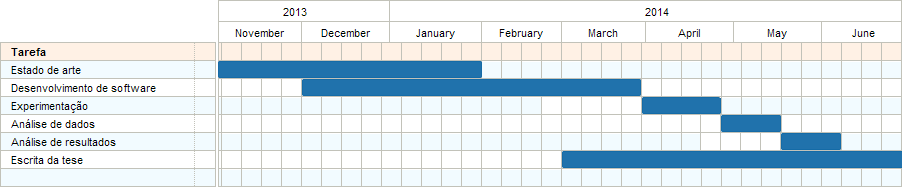
\includegraphics[scale=0.6]{Images/planotese.png}
   \caption{Calendarização através de diagrama de Gantt}
\end{figure}

\section{Ponto de Situação}

Neste momento pode-se considerar que a calendarização definida está a ser cumprida, havendo a registar apenas um ligeiro atraso no que diz respeito ao desenvolvimento do software, sendo esse atualmente o principal foco de atenção. Para além disso, de salientar que o estado de arte, definido como ponto de partida da dissertação, foi efetuado tal como previsto. Foi também submetida uma publicação, para uma conferência internacional, com a proposta de arquitetura. Os próximos passos passam por concluir o desenvolvimento do software, para que seja possível experimentá-lo e efetuar o levantamento de dados.

Posto isto é apresentado o estado quantitativo atual das tarefas definidas no início da dissertação:

\begin{center}
\begin{tabular}{| l | c |}
  \hline
  \textbf{Tarefa} & \textbf{Estado} \\
  \hline
  Estado de arte & 90\%  \\
  \hline
  Desenvolvimento de Software & 30\%  \\
  \hline
  Experimentação & 0\%  \\
  \hline
  Análise de dados & 0\% \\
  \hline
  Análise de resultados & 0\% \\ 
  \hline
  Escrita da tese & 25\% \\
  \hline
\end{tabular}
\end{center}




